% !TEX root = ../Vorlage_DA.tex
%	########################################################
% 							Arbeitstitel
%	########################################################


%	--------------------------------------------------------
% 	Überschrift, Inhaltsverzeichnis
%	--------------------------------------------------------
\chapter*{Thema: \newline \htlArbeitsthema }



%	--------------------------------------------------------
% 	Bearbeiter
%	--------------------------------------------------------
\section*{Subtopics and Editor:}


\textbf{Implementing SLAMS and DeepTAM, Image Pre-Processing}\\ 
Alexander Voglsperger, 5AHELS\\
\emph{Advisors:} Dipl. Ing. Müller Gerhard\\[2ex] 
%
\textbf{Implementing DeepTAM, Gathering Trainingdata}\\ 
Simon Moharitsch, 5AHELS\\
\emph{Advisors:} Dipl. Ing. Müller Gerhard\\[2ex]



%	--------------------------------------------------------
% 	Beteiligte Firmen
%	--------------------------------------------------------
\section*{Projectpartner:}

\renewcommand{\arraystretch}{1.5}
\begin{tabularx}{1\textwidth}{@{} l X @{}}

\emph{Designation:} & Johannes Kepler University - Artificial Intelligence Lab\\
\emph{Address:} & Altenberger Straße 69\\
\emph{ZIP, location:} & 4040 Linz, Austria\\
\emph{Contact person:} & Dr. Nessler Bernhard\\
\emph{Phone:} & +43 (0)732 2468 4539\\
\emph{E-Mail:} & nessler@ml.jku.at\\

\end{tabularx}


%--------------------------------------------------------------------------------
%  Vorgeschriebene Dokumentationsseiten
%--------------------------------------------------------------------------------

\pagebreak
\thispagestyle{empty}
\newgeometry{top=2cm, bottom=1.5cm}

\begin{minipage}[c]{0.20\linewidth}

\includegraphics[width=0.8\linewidth]{media/images/htl_c_cmyk_rein}
\end{minipage}
\begin{minipage}[c]{0.6\linewidth}
\begin{center}
{\bfseries\sffamily\large Höhere  technische  Bundeslehranstalt\\
und  Bundesfachschule  Braunau\\
Elektronik und Technische Informatik\\
{\normalsize School autonomous focus on Mobile Computing and Software Engineering} }
\end{center}
\end{minipage}
\begin{minipage}[c]{0.2\linewidth}
\hfill 
\includegraphics[width=0.8\linewidth]{media/images/htl-bildung-mit-zukunft}
\end{minipage}\\

\vspace{1em}
\begin{center}
\bfseries\sffamily\Large
DIPLOMA DOCUMENTATION
\end{center}
\vspace{1ex}

\renewcommand{\arraystretch}{2}
\begin{tabularx}{1\textwidth}{ p{3.5cm} X }

\textbf{Author} & 
Alexander Voglsperger, Simon Moharitsch \\

\textbf{Vintage\linebreak School year} & 
5AHELS 2019/2020 \\

\textbf{\mbox{Topic of the } \mbox{diploma documentation}} & 
\htlArbeitsthema \\

\textbf{Cooperation\-partner} &
Johannes Kepler University - Artificial Intelligence Lab\\

\textbf{Task definition} & 
{A camera delivers a sequence of 2D pictures of the environment in front of a car. Based on each single picture a so called \gls{slam} (Simultaneous Localization and Mapping) is used to try fetching depth information out of a regular picture that doesn't contain any depth information and generate a 3D map.}\\

\textbf{Realization} & 
{As a foundation the Robot Operating System (\gls{ros}) \ref{ref:ros} is used because it is freely available and has an active community supporting the project. The ORB SLAM and LSD SLAM have already been implemented in ROS as nodes and can be used with changing a few things to get it working. DeepTAM is fairly new and hasn't been implemented in ROS yet.} \\

\textbf{Outcome} & 
{Lorem ipsum dolor sit amet, consetetur sadipscing elitr, sed diam nonumy eirmod tempor invidunt ut labore et dolore magna aliquyam erat, sed diam voluptua. At vero eos et accusam et justo duo dolores et ea rebum. Stet clita kasd gubergren, no sea takimata sanctus est Lorem ipsum dolor sit amet. Lorem ipsum dolor sit amet, consetetur sadipscing elitr, sed diam nonumy eirmod tempor invidunt ut labore et dolore magna aliquyam erat, sed diam voluptua. At vero eos et accusam et justo duo dolores et ea rebum. Stet clita kasd gubergren, no sea takimata sanctus est Lorem ipsum dolor sit amet.} \\

\end{tabularx}

%--------------------------------------------------------------------------------

\pagebreak
\thispagestyle{empty}
\newgeometry{top=2cm, bottom=1.5cm}


\begin{minipage}[c]{0.20\linewidth}

\includegraphics[width=0.8\linewidth]{media/images/htl_c_cmyk_rein}
\end{minipage}
\begin{minipage}[c]{0.6\linewidth}
\begin{center}
{\bfseries\sffamily\large Höhere  technische  Bundeslehranstalt\\
und  Bundesfachschule  Braunau\\
Elektronik und Technische Informatik\\
{\normalsize School autonomous focus on Mobile Computing and Software Engineering} }
\end{center}
\end{minipage}
\begin{minipage}[c]{0.2\linewidth}
\hfill 
\includegraphics[width=0.8\linewidth]{media/images/htl-bildung-mit-zukunft}
\end{minipage}\\

\vspace{1em}

\renewcommand{\arraystretch}{2}
\begin{tabularx}{1\textwidth}{ p{3.5cm} X }

\textbf{\mbox{Illustrative graph,} \mbox{photo} \mbox{(incl. explanation)}} & 
{
Landing page of HTL-carpooling:
\begin{center}
	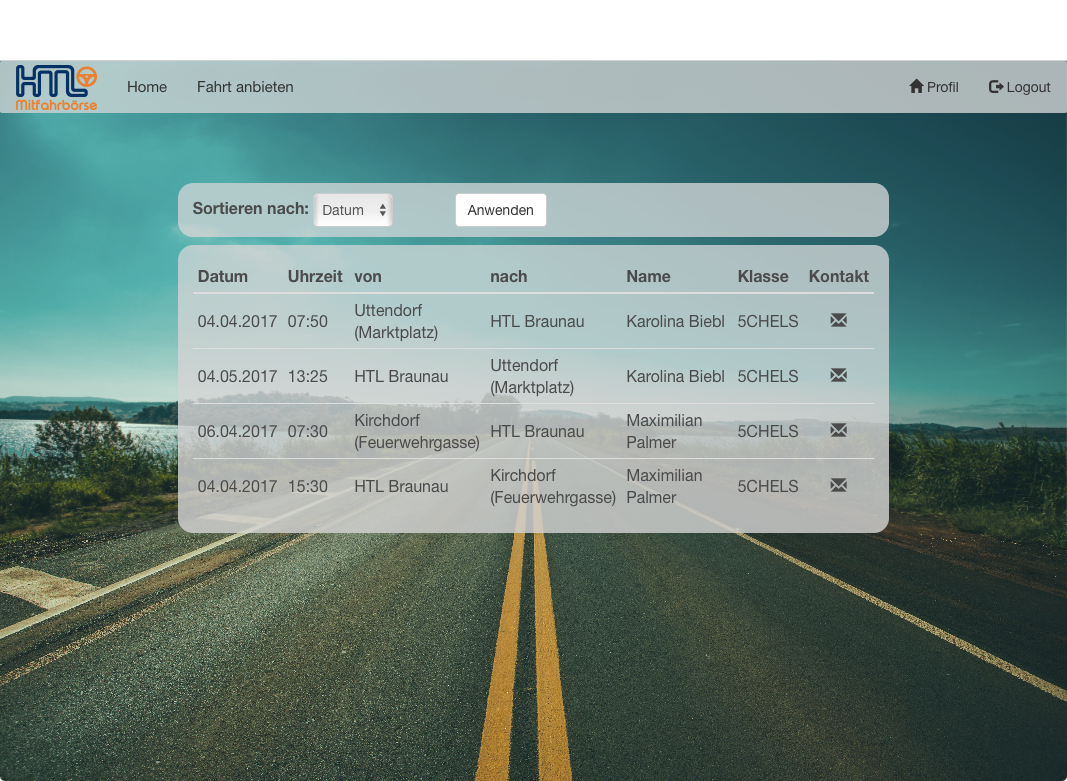
\includegraphics[width=1\linewidth]{media/images/typ_screen}
\end{center}
} \\
  
%\textbf{\mbox{Participation in} competitions, Awards} & 
%{
%Participated:
%\begin{itemize}
%\item Jugend Innovativ
%\item ITs Award
%\item FH Kärnten Maturaprojekt-Wettbewerb
%\item computer creative wettbewerb
%\item 120 Sekunden Wettbewerb
%\end{itemize}
%} \\

\textbf{\mbox{Accessibility of} \mbox{diploma thesis}} & 
{HTL Braunau archive, or\newline \url{https://diplomarbeiten.berufsbildendeschulen.at/}} \\



\end{tabularx}




%--------------------------------------------------------------------------------
% Unterschriften
%--------------------------------------------------------------------------------



\vspace*{\fill}

\textbf{Approval (date / signature)}

\fbox{
\begin{minipage}[t][3cm]{0.5\linewidth}
\centering
Examiner \\
%\hspace*{\fill}\includegraphics[width=0.8\linewidth]{fig/Unterschrift}\hspace*{\fill}
\vfill
\end{minipage}}
\fbox{
\begin{minipage}[t][3cm]{0.5\linewidth}
\centering
Head of College / Department
\vfill
\end{minipage}
}

\restoregeometry

